\chapter{Wymagania i narzędzia}
\label{ch:wymagania-i-narzedzia}

\paragraph{}
Po analizie tematu zdecydowano, że zostanie stworzona aplikacja przeglądarkowa. Będzie się ona składała z trzech warstw: backend, frontend i baza danych. Backend to część funkcjonalna programu, w niej odbywają się obliczenia i logika programu. Frontend odpowiada za interfejs - obsługę formularzy, przycisków, zakładek. Trzecią częścią jest baza danych, która przechowuje dane użytkowników i stworzonych przez nich obiektów. Lokalizatorem, który został wybrany do wspólpracy z programem, jest model Mking MK07A. Spełnia on wymagania urządzenia, które zostały opisane podczas analizy. Ponadto, jest dostępny do kupienia na wielu stronach internetowych. Dodatkowym atutem jest jego akumulator, którego pojemność wynosi 10000 mAh, dzięki czemu nie wymaga częstego ładowania. Zoostał on zakupiony, wraz z kartą SIM, aby możliwe było uruchomienie i skonfigurowanie urządzenia.

\paragraph{}
Tworzona aplikacja ma ułatwić użytkownikowi zarządzanie lokalizatorami, kierowcami i pojazdami jednocześnie oraz pozwalać na wyświetlanie tras poszczególnych kierowców i pojazdów. Wymagania aplikacji należy podzielić na funkcjonalne i niefunkcjonalne. Przyjrzyjmy się w pierwszej kolejności wymaganiom funkcjonalnym. Zdecydowano się na model przypadków użycia, które zostały poniżej przedstawione.

\section{Wymagania funkcjonalne}
\paragraph{}
Dla niezalogowanego użytkownika przewidziano dwa przypadki użycia (przedstawia je diagram widoczny na rys 3.1). Pierwszy to  rejestracja - gdy użytkownik wchodzi na stronę aplikacji, może się zarejestrować, czyli stworzyć bezpłatne konto, które będzie przypisane do podanego przez niego w formularzu rejestracji adresu email. Drugą opcją jest  logowanie. W przypadku uprzedniej rejestracji w systemie, użytkownik może zalogować się na istniejące konto.

\paragraph{}
Przypadków dla zalogowanego użytkownika jest nieco więcej (przedstawia je diagram widoczny na rys 3.2) . Dodanie obiektu składa się z trzech przypadków użycia. Jednym z nich jest dodanie kierowcy, w któym użytkownik ma możliwość dodania kierowcy do swojego konta, podając jego imię oraz nazwisko. Kolejny przypadek to dodanie pojazdu. Pozwala zapisanie w systemie pojazdi poprzez podanie jego marki, modelu, numeru rejestracyjnego oraz numeru VIN. Dodanie lokalizatora to ostatni z przypadków wchodzących w skład dodania obiektu. W tym wypadku użytkownik może dodać posiadane lokalizatory do swojego konta, podając ich nazwę, numer seryjny oraz typ. Poza obiektem, użytkownik może również dodać powiązanie. Jednym z nich jest kierowca pojazdu - ten przypadek umożliwia powiązanie kierowcy z pojazdem w podanym przez użytkownika okresie czasu. Drugie powiązanie to  lokalizator w pojeździe. Działa na podobnej zasadzie, umożliwia powiązanie lokalizatora z pojazdem w danym okresie czasu. Użytkownik będzie w stanie również wyświetlać trasę. Do wyboru jest trasa przebyta przez konkrentego kierowcę, pojazd lub lokalizator. Każda z trzech opcji umożliwia zdefiniowanie okresu czasu, z którego aplikacja ma wyświetlić trasę. Kolejnym przypadkiem jest usunięcie obiektu. Dostępna jest opcja usunięcia kierowcy, pojazdu lub lokalizatora - każda z nich kasuje dany obiekt z systemu. Powiązania również można usunąć, kierowcę pojazdu lub lokalizator w pojeździe, czego następstwem jest brak istnienia tego konkretnego powiązania w aplikacji.

\section{Wymagania niefunkcjonalne}
\paragraph{}
Wymagania niefunkcjonalne definiują w jaki sposób aplikacja powinna działać. Dążąc do jak największej liczby użytkowników, ustalono, iż jednym z tego typu wymagań jest prosta obsługa. Oznacza to przede wszystkim utworzenie intuicyjnego interfejsu. Dostęp do każdej funkcji programu powinien być możliwy przy wykonaniu minimalnej ilości kliknięć myszy (lub ekranu w przypadku urządzeń dotykowych), nieprzekraczającej trzech. Kolejnym założonym wymaganiem są niskie wymagania systemowe - aplikacja powinna być dostępna dla urządzeń posiadających powszechnie używane przeglądarki internetowe, takie jak Chrome, Firefox, Opera czy Safari. Ostatnim wymaganiem niefunkcjonalnym jest skalowalność interfejsu użytkownika. Wymagane jest, aby program był dostosowany do różnej wielkości oraz rozdzielczości ekranów. Użytkowanie aplikacji powinno być możliwe na najpopularniejszych smartfonach, jak na przykład Samsung S24 lub Iphone 15 od Apple.

\begin{figure}
\centering
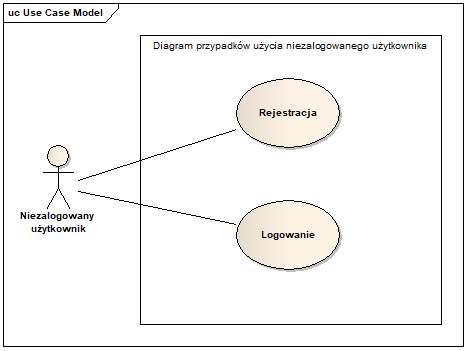
\includegraphics[width=0.6\textwidth]{./graf/Przypadki_uzycia_niezalogowany.png}
\caption{Diagram przypadków użycia niezalogowanego użytkownika.}
\label{fig:3.1}
\end{figure}

\begin{figure}
\centering
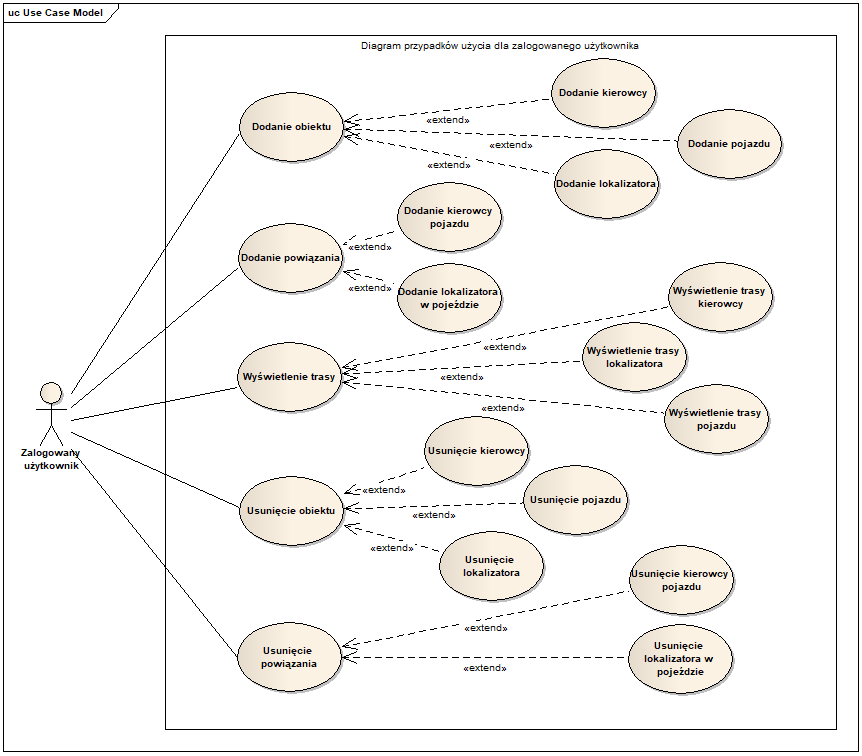
\includegraphics[width=1\textwidth]{./graf/Przypadki_uzycia_zalogowany.png}
\caption{Diagram przypadków użycia zalogowanego użytkownika.}
\label{fig:3.2}
\end{figure}

\section{Stos technologiczny}
\paragraph{}
Przed rozpoaczęciem tworzenia programu, wybrano odpowiednie języki programowania, które umożiwiają budowę aplikacji przeglądarkowej. Zdecydowano się także na biblioteki i platformy programistyczne, które ułatwiają pisanie kodu i komunikacje między różnymi częściami aplikacji.

\subsection{Java}
\paragraph{}
Ze względu na liczne biblioteki usprawniające proces rozwijania oprogramowania, część funkcjonalną programu postanowiono napisać w języku Java. Jest to jeden z najpopularnijeszych wysokopoziomowych języków programowania. Stworzony w 1995 roku, jest nadal rozwijany i powszechnie używany. Jego cechami są przede wszystkim: obiektowość, dobrze rozwinięta biblioteka standardowa, niezliczona ilość dodatkowych bibliotek. Posiada on również Garbage Collector, odpowiadający za zarządzanie pamięcią, co zwiększa bezpieczeństwo języka. Więcej informacji na ten temat można znaleźć w książce "Java. Efektywne programowanie"\ autora Joshua Bloch. Jest to częsty wybór w przypadku tworzenia aplikacji przeglądarkowych, ze względu na istniejące platformy programistyczne oraz biblioteki, będące idealnym rozwiązaniem do tego typu programów.

\subsection{Spring Boot}
\paragraph{}
W celu konfiguracji aplikacji przeglądarkowej została wybrana platforma programistyczna, jaką jest Spring Boot. Jest popularnym wyborem dla języka Java, gdyż w znaczny sposób ułatwia konfigurację tego typu aplikacji, jak również późniejsze jej rozwijanie pod względem tworzenia REST API czy połączenie programu z bazą danych. Konfiguracja odbywa się w dużej mierze automatycznie, wkład programisty opiera się przede wszystkim na dodaniu odpowiednich zależności. Charakterstyczne dla Spring Boot są adnotacje, które są poprzedzone znakiem "@". To dzięki nim Spring Boot potrafi interpretować napisany kod, aby następnie wykonywać pewne operacje automatycznie. Więcej informacji na ten temat znajduje się na oficjalnej stronie producenta.

\subsection{JavaScript}
\paragraph{}
To również bardzo powszechny język programowania, natomiast w odróznieniu do Javy, odpowiada on przede wszystkim za interfejs użytkownika. Ważną jego cechą, wykorzystywaną w aplikacjach przeglądarkowych, jest obługa asynchroniczności. Jest to spowodowane wysyłaniem zapytań HTTP, które trafiają do Javy, a odpowiedzi nie zawsze są natychmiastowe. Więcej opisuje David Flanagan w swojej książce "JavaScript. The Definitive Guide".

\subsection{TypeScript}
\paragraph{}
Nie jest uznawany za osobny język, a za nadzbiór JavaScriptu. Rozszerza jego możliwości, przede wszystkim dzięki typowaniu, które polega na tym, iż zmiennym można przyoisywać konkretny, zdefiniowany typ. Dotyczy to również danych zwracane przez funkcje. Znacznie zwiększa to czytelność kodu oraz pozwala uniknąć przypisywania niewłaściwych typów do zmiennych. Informacje na temat tego języka można znaleźć w oficialnej dokumentacji TypeScript.

\subsection{React}
\paragraph{}
React jest biblioteką do tworzenia interfejsu użytkownika. Działa z językiem JavaScript, jak również TypeScript. Został on stworzony, aby budowane aplikacje przeglądarkowe były dynamiczne - to znaczy aby nie potrzebowały odświeżania strony, aby aktualizować jej widok. React polega na tworzeniu komponentów, które odpowiadają za renderowanie określonej części interfejsu. Charakterystycznymi elementami tej biblioteki są Hooki, czyli funkcje umożliwiające zarządzanie stanem komponentów. Aby dowiedzieć się więcej, warto wejść na oficjalną stronę internetową React.

\subsection{PostgreSQL}
\paragraph{}
Zaawansowany system do zarządzania bazą danych, zgodny ze standardem SQL, pozwalający również na dostosowanie do indywidualnych potrzeb, gdyż posiada na przykład możliwość tworzenia własnych typów danych. Często wykorzystywany w aplikacjach przeglądarkowych, ze względu na jego wysoką wydajność oraz skalowalność. Dokumentację do PostgreSQL można pobrać z oficjalnej strony.

\subsection{PostGIS}
\paragraph{} 
Jest to rozszerzenie do PostgreSQL, które wspiera obsługę danych geograficznych i przestrzennych. Daje możliwość przechowywania danych przede wszystkim o punktach, ale również o liniach, wielokątach. Rozszerzenie to jest używane w przypadku programów związanych z obsługą GPS oraz map, także idealnie pasuje do niniejszej pracy. Dokumentacja dostępna na oficjalnej stronie PostGIS.

\subsection{Hibernate}
\paragraph{}
Bardzo często wybierana platforma programistyczna w celu automatyzacji mapowania między obiektami w języku Java, a tabelami w bazie danych. Umożliwia to pracę nad obiektami, bez konieczności wykonywania skomplikowanych zapytań SQL. Więcej informacji znajduje się na oficjalnej stronie internetowej Hibernate.

\subsection{Git}
Ostatnim elementem jest system kontroli wersji. Dzięki temu postępy w pracy będą zabezpieczone. Niemniej jednak, to nie jedyny atut. W przypadku błędów aplikacji spowodowanych zmianami w kodzie źródłowym, zlokalizowanie ich przyczyny będzie znacznie ułatwione. Wybrano system Git, gdyż jest on najpopularniejszą opcją, a co za tym idzie, jest obsługiwany przez niemal każde oprogramowanie programistyczne. Dokumentacja do tego systemu widnieje na oficjalnej stronie Git.

\section{Oprogramowanie do edycji kodu}
\paragraph{}
Aby przystąpić do pisania kodu, należało wybrać i zainstalować odpowiednie programy, które to wspierają odpowiednie języki, biblioteki czy platformy programistyczne.

\subsection{IntelliJ Idea}
\paragraph{}
Do części funkcjonalnej został wykorzystany Intellij Idea wydawcy JetBrains. Ten program jest zaawansowanym, wieloplatformowym środowiskiem programistycznym, posiadającym dużą ilość wbudowanych narzędzi, jak również obsługującym wiele bibliotek i platform programistycznych, takich jak Spring Boot. Hibernate oraz JPA również są wspierane przez Intellij. Są to narzędzia, które potrafią powiązać kod aplikacji z bazą danych, co znacznie uprości rozwijanie programu.

\subsection{Visual Studio Code}
\paragraph{}
Przechodząc do interfejsu użytkownika, a zatem do kodu w języku TypeScript z zastosowaniem biblioteki React, wybrano Microsoft Visual Studio Code, który jest powszechnie używany przez programistów w tym celu, ze względu na odpowiednie wsparcie języków i bibliotek typowych do tworzenia wizualnej części aplikacji. 

\subsection{PgAdmin}
\paragraph{}
W kontekście bazy danych, potrzebne było oprogramowanie, które będzie w stanie obsługiwać zapytania kierowane do bazy danych - na początku do stworzenia bazy, poszczególnych tabel, a w przyszłości do eliminowania ewentualnych błędów oraz do testowania aplikacji. PgAdmin umożliwia te operacje, jak również pozwala na stworzenie diagramu bazy danych.

\subsection{GitHub}
\paragraph{}
Należało również dokonać wyboru platformy hostingowej, która będzie przechowywała repozytorium Git. W tym celu skorzystano z GitHuba, będącego jedną z najbardziej powszechnych opcji. Jest on także wspierany przez większość środowisk programistycznych.

\section{Metodyka pracy}

\paragraph{}
Do usystematyzowania i organizacji prac nad projektem wybrano model kaskadowy (ang. waterfall). Polega on na sekwencyjnym działaniu nad kolejnymi etapami. Zdecydowano się na niego, ponieważ w opinii autora, w przypadku jednoosobowego projektu, umożliwia on zoptymalizownie wykorzystywanego czasu. Zrezygnowano z innych opcji metodyki pracy, wśród których przykładem jest Scrum. Sprawdza się on przede wszystkim w przypadku pracy w zespole, zatem uznano, że nie nadaje się do tego projektu.
